% Name: Nondeterministic finite automaton
% Description: An NFA with epsilon transitions.
% Tags: NFA, epsilon transition, nondeterministic

\usetikzlibrary{automata, positioning}

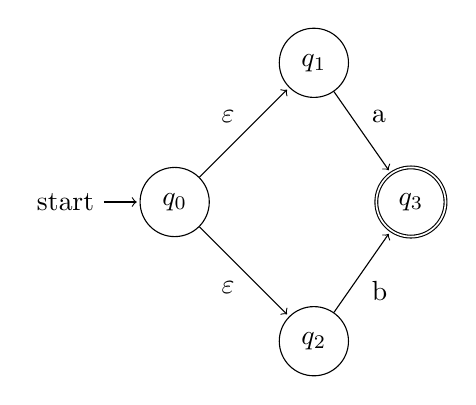
\begin{tikzpicture}[shorten >=1pt, node distance=2.5cm, on grid, auto]
  \node[state, initial] (q0) {$q_0$};
  \node[state] (q1) [above right=of q0] {$q_1$};
  \node[state] (q2) [below right=of q0] {$q_2$};
  \node[state, accepting] (q3) [right=3cm of q0] {$q_3$};

  \path[->]
    (q0) edge node{$\varepsilon$} (q1)
         edge node[below left]{$\varepsilon$} (q2)
    (q1) edge node{a} (q3)
    (q2) edge node[below right]{b} (q3);
\end{tikzpicture}
